 %-------------------------------------------------------------------------------
%-------------------------------------------------------------------------------
%-------------------------------------------------------------------------------
\chapter{Systèmes différentiels}
%-------------------------------------------------------------------------------
%-------------------------------------------------------------------------------
\thispagestyle{empty}
\begin{abstract}
\begin{itemize}
    \item Dans le TP nous allons prolonger l'étude des équations différentielles en quittant le cas des équations scalaires d'ordre 1.
    \item Dans un premier temps nous allons voir qu'il n'y a rien à changer quand on a plusieurs équations différentielles couplées : les dérivées des fonctions varient en fonction des valeurs de {\bf plusieurs} fonctions inconnues.
    \item Nous verrons ensuite comment se ramener au cas précédent dans le cas d'équations d'ordre 2 ou plus.
\end{itemize}
\end{abstract}
%-------------------------------------------------------------------------------
%-------------------------------------------------------------------------------
%-------------------------------------------------------------------------------
\section{Complément de cours}
%-------------------------------------------------------------------------------
%-------------------------------------------------------------------------------
%-------------------------------------------------------------------------------
\subsection{Présentation}
%-------------------------------------------------------------------------------
%-------------------------------------------------------------------------------
Il arrivera souvent que les modélisations des phénomènes aboutissent à plusieurs fonctions inconnues solutions différentielles dans lesquelles plusieurs fonctions interviennent, des systèmes différentiels. Par exemple Lorenz, en simplifiant des équations intervenant en météorologie, est parvenu au système 
\[\left\{\begin{matrix}x'&=&\sigma(y-x)\\ y' &=& \rho x - y - xz\\
z'&=& xy - \beta z\\
\end{matrix}\right.\]

Dans certains cas (rares) le sens physique ou chimique permet de détecter des symétries qui, après changement de variables, permettent de découpler les équations et d'obtenir plusieurs équations d'ordre 1 simple. Ce sera aussi le cas dans le cas de systèmes linéaires à coefficients constants dont l'étude sera vue en mathématiques et utilise la diagonalisation.

Par exemple $\left\{\begin{matrix}x'&=&2x + 2y\\ y' &=& x + 3 y\\ \end{matrix}\right.$ se transforme en
$\left\{\begin{matrix}u'&=&4u\\ v' &=& v\\ \end{matrix}\right.$ en posant $u = 2+2y$ et $v =x-y$.
%-------------------------------------------------------------------------------
%-------------------------------------------------------------------------------
\subsection{Une idée}
%-------------------------------------------------------------------------------
%-------------------------------------------------------------------------------
Nous allons ici donner une méthode qui permettra de résoudre numériquement, c'est-à-dire de manière approchée, les systèmes différentiels généraux. 

L'idée est de considérer les différentes équations dans leur ensemble en formant la fonction {\bf vectorielle} qui rassemble des fonctions inconnues. Dans le cas des équations de Lorenz, on pose $M(t) = \bigl(x(t), y(t), z(t)\bigr)$.

La dérivée de la fonction vectorielle est le vecteur dont les composantes sont les dérivées, il s'exprime donc en fonction de la fonction initiale et du temps (le temps n'apparaît pas toujours).
\[M'(t) = \varphi\bigl(M(t), t\bigr)\]

On est ramené à ce que l'on connaît déjà, avec la nouveauté que les fonctions inconnues sont à valeurs dans un ensemble $\R^n$ et que la première variable de $\varphi$ appartient à cet espace $\R^n$.

\medskip

La méthode d'Euler s'applique toujours : $M(t_{k+1})\sim M(t_k) + (t_{k+1} - t_k) M'(t_k)$.

Cependant les opérations qui interviennent ici sont l'addition de deux vecteurs et le produit d'un vecteur par un scalaire, ce sont les opérations définie dans tout espace vectoriel.
%-------------------------------------------------------------------------------
%-------------------------------------------------------------------------------
\subsection{Des vecteurs en Python}
%-------------------------------------------------------------------------------
%-------------------------------------------------------------------------------
Un moyen naturel de rassembler plusieurs valeurs en Python est d'utiliser une liste.

Par exemple, dans le cas des équations de Lorenz, on travaille avec des objet des la forme \type{[x, y, z]}. Malheureusement l'addition de deux listes et le produit d'une liste (seulement par un entier) ne sont pas les opérations souhaitées.
On pourrait les définir "à la main".

Heureusement, il existe le module \Type{numpy} :
%-------------------------------------------------------------------------------
\begin{lstlisting}
import numpy as np
\end{lstlisting} 
%-------------------------------------------------------------------------------

Il définit un type de données, \Type{array}, qu'on nommera vecteur.

Si \type{U} est un vecteur, il ressemble beaucoup à une liste Python :
%--------------------------------------------------------------------------
\begin{itemize}
\item on accède et on modifie les éléments par leur indice : \type{U[i] = }, \type{x = U[i]},
\item la longueur du tableau est définie par \type{len(U)},
\item on peut parcourir les éléments par \type{for u in U},
\item on peut extraire des sous-vecteurs : \type{U[i : j]}
\end{itemize}
%--------------------------------------------------------------------------

On définit un vecteur
%--------------------------------------------------------------------------
\begin{itemize}
\item soit en convertissant une liste, \type{U = np.array(L)}
\item soit en définissant un tableau de valeurs nulles, \type{U = np.zeros(n)} puis en le remplissant.
\item {\bf On ne peut pas construire un vecteur par adjonctions, par de méthode \type{append}}.
\end{itemize}
%--------------------------------------------------------------------------

\medskip

Ensuite les vecteurs réagissent à l'addition et à la multiplication par un scalaire comme des vecteurs d'un espace vectoriel.
%--------------------------------------------------------------------------
\begin{lstlisting}
>>> a = np.array([1.0, 3.5, -1.2])
>>> b = np.array([2.1, 0.3, 12.4])
>>> a + 1.75*b
array([ 4.675,  4.025, 20.5  ])
\end{lstlisting} 
%-------------------------------------------------------------------------------
%-------------------------------------------------------------------------------
\subsection{Résolution}
%-------------------------------------------------------------------------------
%-------------------------------------------------------------------------------
Pour résoudre un système différentiel, il y a donc peu de choses qui changent.
%--------------------------------------------------------------------------
\begin{itemize}
\item On définit la fonction qui décrit le système différentiel \type{phi(u, t)} mais \type{u} sera un vecteur de longueur $n$, le nombre de variables et la fonction renvoie un vecteur de même taille.
%--------------------------------------------------------------------------
\begin{lstlisting}
def phi(u, t):
    x, y, ... = u
    x_prime = ...
    y_prime = ...
    ...
    return np.array([x_prime, y_prime, ...])
\end{lstlisting} 
%-------------------------------------------------------------------------------
\item La condition initiale est un vecteur dont les composantes sont les valeurs et $t_0$ de chacune des variables.
\item La liste des temps est identique ; on pourra utiliser \type{np.linspace(a, b, n)} qui construit un vecteur de taille $n$ dont les valeurs vont de $a$ à $b$ compris et sont régulièrement espacées.  
\item On utilise les fonctions de résolution, \type{euler} ou autre {\bf sans rien changer.}
\end{itemize}
%-------------------------------------------------------------------------------
%-------------------------------------------------------------------------------
\subsection{Un exemple}
%-------------------------------------------------------------------------------
%-------------------------------------------------------------------------------
\begin{enumerate}
\item On se donne le système différentiel 
\[\left\{\begin{matrix}x'&=&\frac{xy}{x^2 + y^2}\\ y' &=& \frac{y^2 +a^2 - ax}{x^2 + y^2}\\
\end{matrix}\right.\]

On pourra choisir $a= 1$. 
%-------------------------------------------------------------------------------
\item On commence par définir la fonction $\varphi$.

\begin{lstlisting}
a = 1

def phi(u, t):
    x, y = u
    den = x**2 + y**2
    dx = x*y/den
    dy = (y**2 + a**2 - a*x)/den
    return np.array([dx, dy])
\end{lstlisting}
%-------------------------------------------------------------------------------
\item On définit ensuite la condition initiale en $t=0$ : \type{u0 = np.array([0.5, 0.0])},
%-------------------------------------------------------------------------------
\item puis une liste de temps : 2000 points sur $[0; 5]$.
\begin{lstlisting}
t_max = 5
N = 2000
T = np.linspace(0, t_max, N)
\end{lstlisting}
%-------------------------------------------------------------------------------
\item On peut alors calculer les solutions : \type{U = euler(phi, u0, T)}
%-------------------------------------------------------------------------------
\item \type{U} est une liste de vecteurs de taille 2, on isole les composantes.
\begin{lstlisting}
X = [u[0] for u in U]
Y = [u[1] for u in U]
\end{lstlisting}
%-------------------------------------------------------------------------------
\item On peut alors tracer les solutions 
\begin{lstlisting}
plt.plot(T, X, label = "x(t)")
plt.plot(T, Y, label = "y(t)")
plt.legend()
plt.show()
\end{lstlisting}
%-------------------------------------------------------------------------------
\item Comme les variables représentent des coordonnées, on peut utilement ici tracer la trajectoire
\begin{lstlisting}
plt.plot(X, Y)
plt.show()
\end{lstlisting}
%-------------------------------------------------------------------------------
\begin{center}
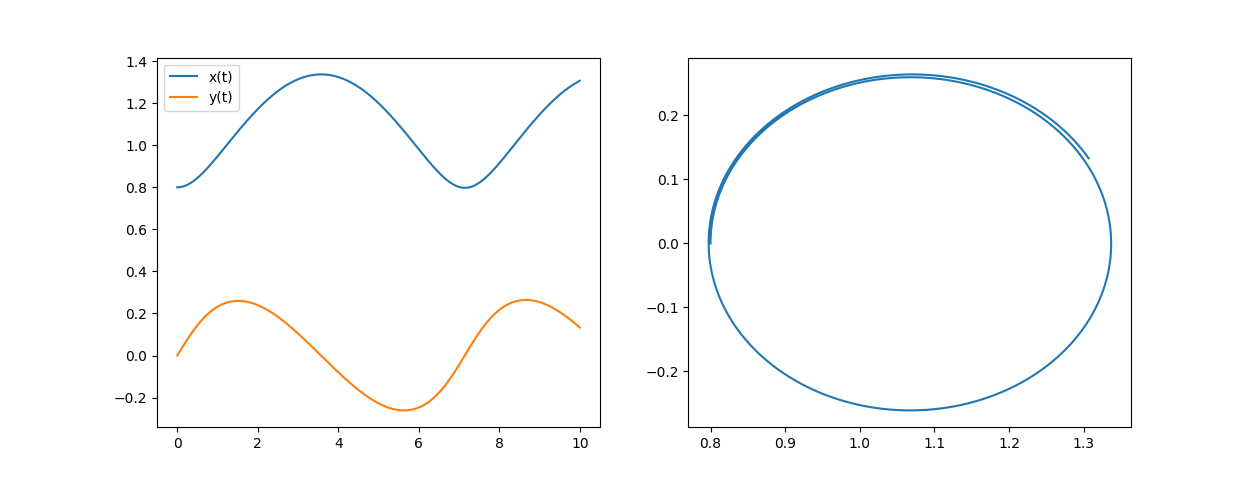
\includegraphics[width=17cm]{euler_vect_ex.png}
\end{center}
%-------------------------------------------------------------------------------
%-------------------------------------------------------------------------------
\begin{minipage}{0.60\linewidth}
\item En théorie, les trajectoires bornées se referment. 

Le graphe ci-dessus présente une divergence. 

On peut obtenir une meilleure approximation en augmentant le nombre de points.

On peut aussi utiliser une méthode plus précise ou, plus simplement, utiliser la fonction \type{odeint} qui s'emploie exactement de la même façon que \type{euler}.
\begin{lstlisting}
from scipy.integrate import odeint
\end{lstlisting}
%-------------------------------------------------------------------------------
\item On rappelle qu'on peut tracer les graphes sur $[-t_{Max} ; 0]$ avec la même condition initiale en définissant une liste de temps à l'envers :
\begin{lstlisting}
T = np.linspace(0, -t_max, N)
\end{lstlisting}
%-------------------------------------------------------------------------------
\item Pour calculer plusieurs solution, par exemple avec des conditions initiales distinctes, on peut inclure les calculs dans une boucle.
\begin{lstlisting}
for x0 in (range(1, 10)):
    x0 = i*a/10
    u0 = np.array([x0 , 0])
\end{lstlisting}
Dans cette exemple on obtient des coniques de mêmes foyer et directrices.
%-------------------------------------------------------------------------------
\end{minipage}
%-------------------------------------------------------------------------------
\hfill
%-------------------------------------------------------------------------------
\begin{minipage}{0.35\linewidth}
\vspace{0pt}
\begin{center}
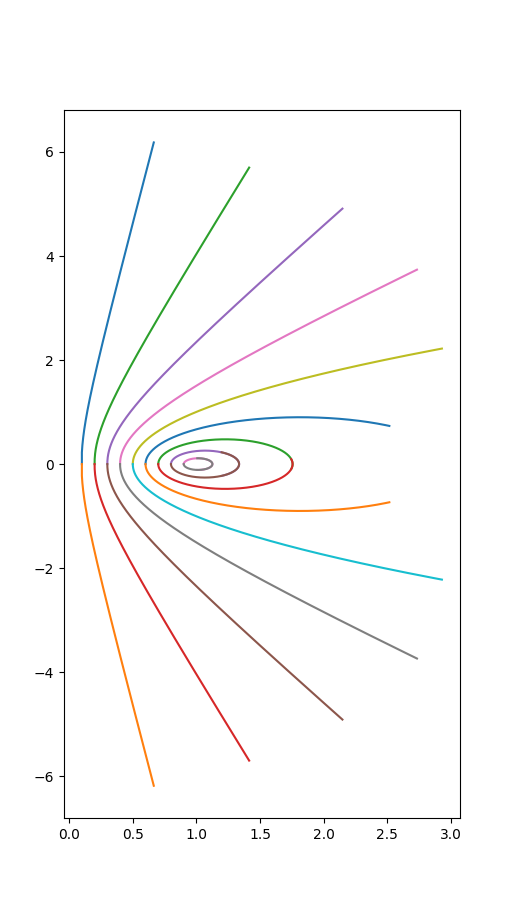
\includegraphics[width=6cm]{euler_vect_multi.png}
\end{center}
\end{minipage}
%-------------------------------------------------------------------------------
\end{enumerate}
%-------------------------------------------------------------------------------
%-------------------------------------------------------------------------------
\subsection{Équations d'ordre 2}
%-------------------------------------------------------------------------------
%-------------------------------------------------------------------------------
Pour résoudre des équations d'ordre 2, on peut modifier la méthode d'Euler en calculant les valeurs de la fonction et celles de sa dérivée. Pour l'équation $y'' = \psi(y, y', t)$, on note $v(t) = y'(t)$ et on a alors 
$v'(t) = y''(t) = \psi\bigl(y(t), y'(t), t\bigr)$.

On aboutit ainsi à un système $\left\{\begin{matrix}y'&=&2v\\ v' &=& \psi(y, y', t)\\ \end{matrix}\right.$

%-------------------------------------------------------------------------------
\begin{minipage}{0.50\linewidth}
{\bf Exemple} : $y''+y'+10y = t$, $y(0)=1$, $y'(0) = 0$.
\begin{lstlisting}
def phi(u, t):
    y, v = u
    acc = t - 10*y - v
    return np.array([v, acc])

u0 = np.array([1, 0])
T = np.linspace(0, 10, 2000)
U = euler(phi, u0, T)
Y = [u[0] for u in U]
plt.plot(T, Y)
\end{lstlisting}
\end{minipage}
%-------------------------------------------------------------------------------
\begin{minipage}{0.35\linewidth}
\begin{center}
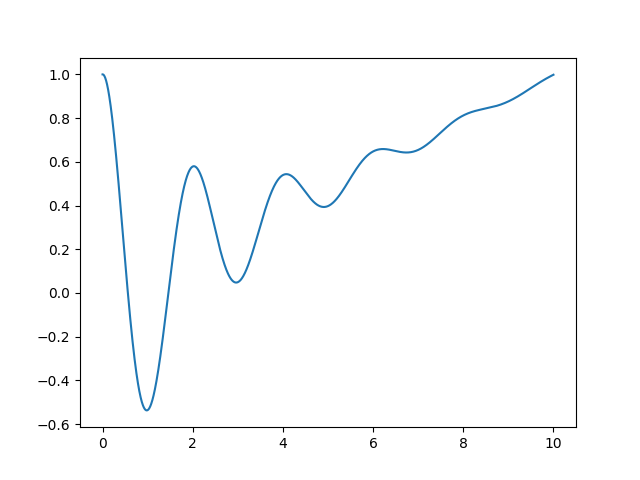
\includegraphics[width=8cm]{euler_vect_2.png}
\end{center}
\end{minipage} 
%-------------------------------------------------------------------------------
\newpage
%-------------------------------------------------------------------------------
%-------------------------------------------------------------------------------
%-------------------------------------------------------------------------------
\section{Exercices}
%-------------------------------------------------------------------------------
%-------------------------------------------------------------------------------
%-------------------------------------------------------------------------------
\subsection{Proies-prédateurs}
%-------------------------------------------------------------------------------
%-------------------------------------------------------------------------------
\begin{minipage}{0.50\linewidth}
Un système classique pour modéliser les interactions entre proies et prédateurs a été obtenu par Lotka et Volterra qui voulaient comprendre les évolutions des populations de requeins et de thon en Adriatique après la première guerre mondiale. Après simplification des constantes on arrive au système suivant.

$\displaystyle \left\{\begin{matrix}x'&=&x-xy\\ y' &=& xy - y\\\end{matrix}\right.$.

%--------------------------------------------------------------------------
%--------------------------------------------------------------------------
\begin{Exercise}\it 
Tracer les solutions de solutions du système pour différentes conditions initiales $(a,1)$ avec $a> 1$ sur $[0; 20]$
\end{Exercise}
%--------------------------------------------------------------------------
\begin{Answer}
\begin{lstlisting}
def proiesp(u,t):
  x, y = u
  dx = x - x*y
  dy = x*y - y
  return np.array([dx, dy])

T = np.linspace(0, 10, 1000)
for i in range(6):
  y0 = np.array([1.3 + 0.5*i, 1.0])
  U = odeint(proiesp,y0,T)
  X = [u[0] for u in U]
  Y = [u[1] for u in U]
  plt.plot(X, Y)
plt.show()
\end{lstlisting}
\end{Answer}
%--------------------------------------------------------------------------
\end{minipage}
%-------------------------------------------------------------------------------
\begin{minipage}{0.45\linewidth}
\begin{center}
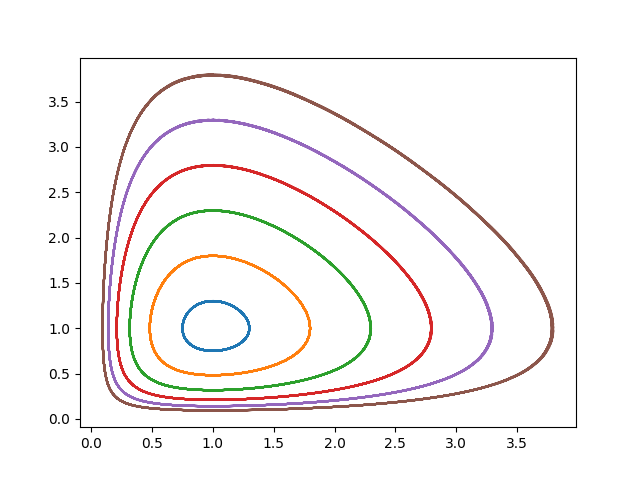
\includegraphics[width=8cm]{euler_vect_proiesp}    
\end{center}
\end{minipage}
%-------------------------------------------------------------------------------
%-------------------------------------------------------------------------------
\subsection{Simulation d'une épidémie}
%-------------------------------------------------------------------------------
%-------------------------------------------------------------------------------
On modélise la propagation d'une épidémie en séparant la population en 3 :
\begin{itemize}
    \item les individus {\bf sains} dont la proportion est représentée par une fonction $S(t)$,
    \item les personnes {\bf infectées} de proportion $I(t)$ et
    \item les guéris comptés par $R(t)$ (pour {\bf recovered}).
\end{itemize}
On parle du modèle SIR.

On définit deux constantes $\beta$ et $\gamma$ qui représente le taux de transmission pour $\beta$, c’est à dire le taux de personnes saines qui deviennent infectées par contact avec les personnes infectées par unité de temps et le taux de guérison pour $\gamma$, c’est à dire le taux de personnes infectées qui deviennent guéries par unité de temps. 

On suppose que les personnes guéries ne peuvent plus être infectées.

Mathématiquement, le modèle SIR est donné par le système suivant :
$\left\{\begin{matrix}
\displaystyle \frac{\d S}{\d t}(t)&=&-\beta S(t)I(t)&&\\ 
\displaystyle \frac{\d I}{\d t}(t)&=&\beta S(t)I(t)&-&\gamma I(t)\\ 
\displaystyle \frac{\d R}{\d t}(t)&=&&&\gamma I(t)\\ 
\end{matrix}\right.$

On note $R_0$ le rapport $\displaystyle \frac \beta\gamma$, il mesure la propagabilité de la maladie.

On prendra comme valeurs $R_0 = 3$ et $\gamma = 0.03$.

On considérera qu'on a $I(0) = 10^{-3}$ et $R(0) = 0$ et on étudiera pour $t\in [0;300]$

%--------------------------------------------------------------------------
%--------------------------------------------------------------------------
\begin{Exercise}\it 
Tracer, sur un même graphique, les proportions de chaque type de population.
\end{Exercise}
%--------------------------------------------------------------------------
\begin{Answer}
\begin{lstlisting}
R0 = 3
gamma = 0.03
beta = R0*gamma

def phi(u, t):
    s, i, r = u
    return np.array([-beta*s*i, beta*s*i - gamma*i, gamma*i])

prop = 1e-3
CI = np.array([1-prop, prop, 0])
t_max = 300
T = np.linspace(0, t_max, 10000)
U = odeint(psi3, CI, T)
S = [u[0] for u in U]
I = [u[1] for u in U]
R = [u[2] for u in U]
plt.plot(T, S, label = "S")
plt.plot(T, I, label = "I")
plt.plot(T, R, label = "R")
plt.legend()
plt.show()
\end{lstlisting}
\newpage
\end{Answer}
%-------------------------------------------------------------------------------
%--------------------------------------------------------------------------
\begin{center}
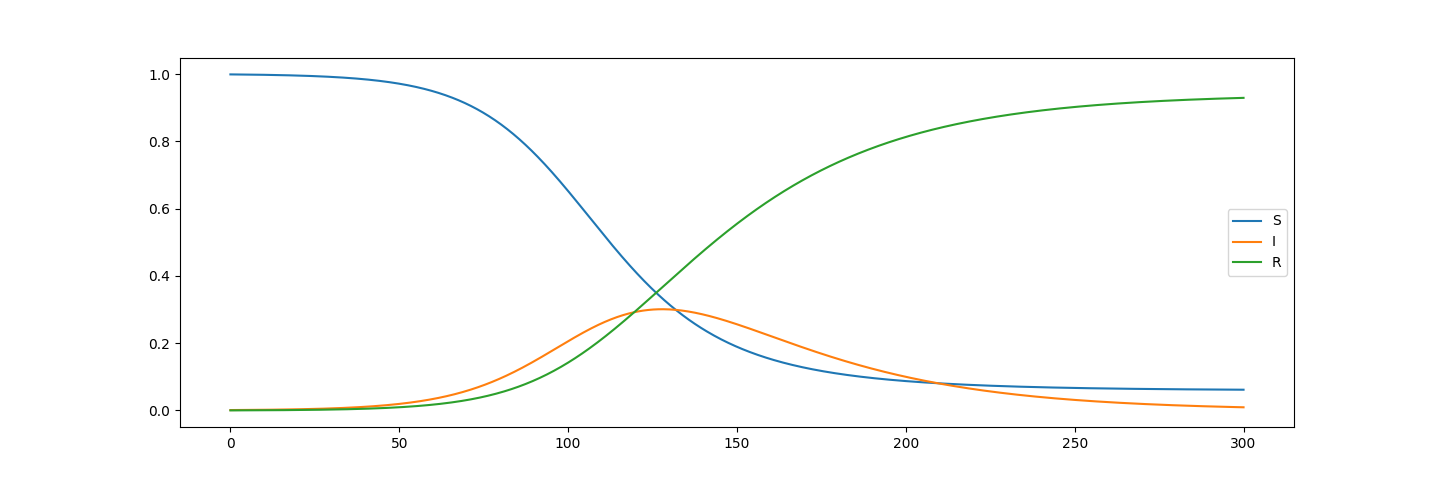
\includegraphics[width=14cm]{euler_vect_SIR}
\end{center}
%-------------------------------------------------------------------------------
On ajoute une période de confinement entre les temps $t= 80$ et $t = 140$, pendant laquelle le coefficient $R_0$ est divisé par 4.
%--------------------------------------------------------------------------
%--------------------------------------------------------------------------
\begin{Exercise}\it 
Après avoir défini une nouvelle fonction $\psi$, tracer, sur un même graphique, les proportions de chaque type de population.
\end{Exercise}
%--------------------------------------------------------------------------
\begin{Answer}
\begin{lstlisting}
def phi(u, t):
    if 10 < t < 40:
        beta1 = beta/2
    else:
        beta1 = beta
    s, i, r = u
    return np.array([-beta1*s*i, beta1*s*i - gamma*i, gamma*i])

prop = 1e-3
CI = np.array([1-prop, prop, 0])

t_max = 100
T = np.linspace(0, t_max, 10000)
U = odeint(psi3, CI, T)
plt.plot(T,U)
plt.show()
\end{lstlisting}
\end{Answer}
%-------------------------------------------------------------------------------
%-------------------------------------------------------------------------------
\begin{center}
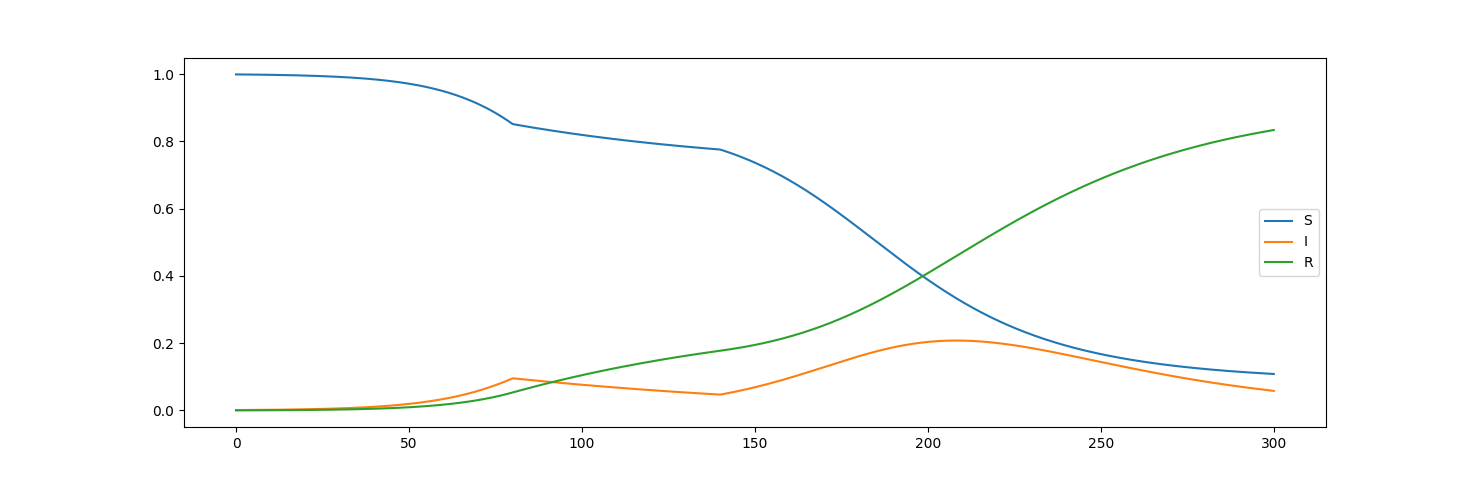
\includegraphics[width=14cm]{euler_vect_SIR_c}
\end{center}
%-------------------------------------------------------------------------------
%--------------------------------------------------------------------------
\subsection{Équations de Lorenz}
%-------------------------------------------------------------------------------
%-------------------------------------------------------------------------------
\begin{minipage}{0.50\linewidth}
Lors de l'étude des phénomènes météorologiques, Edward Lorenz a proposé, en 1963, les équations issues de la mécanique des fluides en un système dynamique tridimensionnel. Ce système engendre un comportement chaotique dans certaines conditions. Il est donné par
\[\left\{\begin{matrix}
x'&=&\sigma(y-x)\\ 
y' &=& \rho x - y - xz\\
z'&=& xy - \beta z\\
\end{matrix}\right.\]
avec $\sigma = 10$, $\rho = 28$ et $\beta = 8/3$.
%-------------------------------------------------------------------------------
%-------------------------------------------------------------------------------
\begin{Exercise}\it
Tracer le portrait de phase sur $[0;30]$ pour les conditions initiales $x(0) =0.1$, $y(0) =0$ et $z(0) =0.1$.
\end{Exercise}
%--------------------------------------------------------------------------
\begin{Answer}
\begin{lstlisting}
def lorenz(u, t):
    sigma = 10
    rho = 28
    beta = 8/3
    x, y, z = u
    vx = sigma*(y - x)
    vy = rho*x - y - x*z
    vz = x*y - beta*z
    return np.array([vx, vy, vz])

T = np.linspace(0, 30, 3000)
y0 = np.array([0.1, 0.0, 0.1])
U = odeint(lorenz, y0, T)
X = [u[0] for u in U]
Y = [u[1] for u in U]
Z = [u[2] for u in U]
dessin = Axes3D(plt.figure()) 
dessin.plot(X, Y, Z) 
plt.show()
\end{lstlisting}
\newpage
\end{Answer}
%--------------------------------------------------------------------------
%--------------------------------------------------------------------------
On pourra tracer une représentation en 3 dimension par
%--------------------------------------------------------------------------
\begin{lstlisting}
from mpl_toolkits.mplot3d import Axes3D
# Un cadre contenant les tracés
dessin = Axes3D(plt.figure()) 
# On y ajoute un tracé
dessin.plot(x, y, z) 
\end{lstlisting}
%--------------------------------------------------------------------------
\end{minipage}
%-------------------------------------------------------------------------------
\begin{minipage}{0.45\linewidth}
\begin{center}
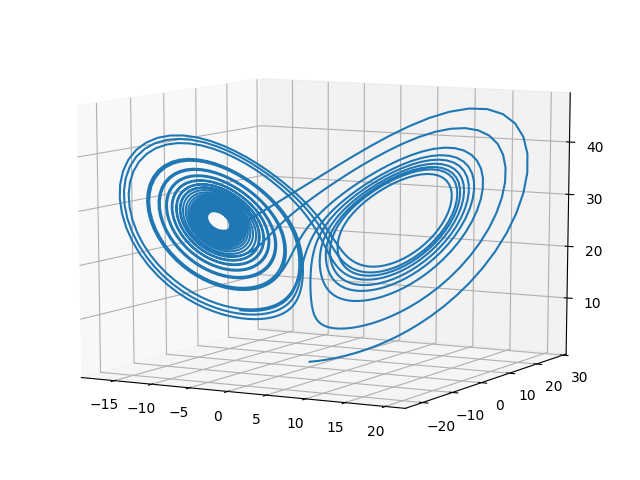
\includegraphics[width=8cm]{euler_vect_Lorenz1}

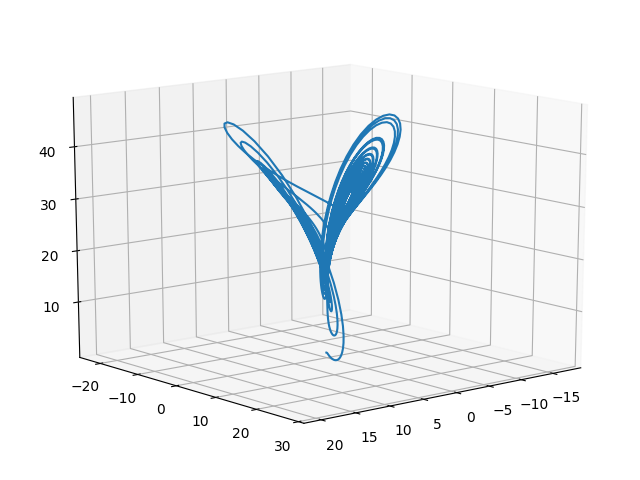
\includegraphics[width=8cm]{euler_vect_Lorenz2}    
\end{center}
\end{minipage}
%-------------------------------------------------------------------------------
%--------------------------------------------------------------------------
\subsection{Équations d'ordre 2}
%-------------------------------------------------------------------------------
%-------------------------------------------------------------------------------
\begin{Exercise}
\it Tracer les solutions de 
$y'' = -2y'+3y$ avec $y(0)=1$ et $y'(0) = -3$. 

Remarquez et essayez d'expliquer ce qui se passe pour les grandes valeurs de $t$.
\end{Exercise}
%--------------------------------------------------------------------------
\begin{Answer}
La solution devrait être $y(t) = e^{-3t}$ mais les erreurs d'arrondi et d'imprécision font que la solution calculée comporte un terme en $e^t$.
\end{Answer}
%--------------------------------------------------------------------------
%--------------------------------------------------------------------------
\begin{Exercise}\it 
Tracer les solutions de l'équation de van der Pol :
$y'' = (1-y^2)y'-y$ pour différentes conditions initiales, par exemple $y_0 = \frac k2$, $y'_0=0$ pour $k\in\{0,1,\ldots, 9\}$.

On pourra tracer la trajectoire dans l'espace des phases $(y, y')$. Que remarque-t-on ?
\end{Exercise}
%--------------------------------------------------------------------------
\begin{Answer}
\begin{lstlisting}
def vdPol(u,t) :
  (x,y) = u
  xPrime = y
  yPrime = y*(1-x*x)-x
  return np.array([xPrime, yPrime])

T = np.linspace(0, 30, 1000)
for i in range(10):
  y0 = np.array([i/2, i/3])
  sol = heun(vdPol, y0, T)
  X = [u[0] for u in sol]
  X = [u[0] for u in sol]
  plt.plot(T, X)
plt.show()
\end{lstlisting}

Toutes les solutions se rapprochent d'un cycle limite.
\end{Answer}
%--------------------------------------------------------------------------
%-------------------------------------------------------------------------------
\subsection{Effet Zeeman}
%-------------------------------------------------------------------------------
%-------------------------------------------------------------------------------
L'électron dans l'atome est classiquement modélisé comme «élastiquement lié» : un point matériel de masse $m$ et de charge électrique $e$, repéré par sa position $\vec{r}$, et soumis de la part du noyau à une force de rappel élastique, anticolinéaire à $\vec{r}$. Il se comporte alors comme un oscillateur harmonique de pulsation $\omega_0$.

Si l'atome est soumis à un champ magnétique $\vec{B}$ colinéaire à $\vec{u}_z$, il subit une seconde force d'origine magnétique ; il se produit alors un phénomène appelé effet Zeeman :
	\begin{itemize}
	\item L'électron garde un mouvement oscillant à la pulsation $\omega_0$ le long du champ magnétique.
	\item Il développe un mouvement bi-harmonique dans le plan perpendiculaire au champ magnétique, aux pulsations $\omega_0\pm\Omega$, où $\Omega$ est une pulsation proportionnelle au champ magnétique.
	\item L'atome peut alors émettre un rayonnement sur les trois pulsations $\omega_0$, $\omega_0-\Omega$ et $\omega_0+\Omega$.
	\end{itemize}
Le mouvement suivant $z$ est un simple oscillateur harmonique découplé des deux autres, donc il ne sera pas étudié.

%-------------------------------------------------------------------------------
\begin{minipage}{0.6\linewidth}
L'équation différentielle gouvernant le vecteur position est 
$\vec{r}\,''(t)+e\vec{r}\,'(r)\wedge\vec{B}+\omega_0^2\vec{r}=\vec{0}$.
Elle se traduit en le système
$\left\{\begin{matrix}
\ddot{x}+\omega_0^2x &=& -2\Omega\dot{y}\\ 
\ddot{y}+\omega_0^2y &=& 2\Omega\dot{x}
\end{matrix}\right.$
avec $\Omega=\frac{eB}{2m}$.

L'équation différentielle portera donc sur 4 variables :
\begin{lstlisting}
def psi4(u, t):
    x, y, vx, vy = u
    ...
\end{lstlisting}


On choisit, pour conditions initiales, $\vec{r}(0)=-a\cos(\theta_0)\vec{u}_y$ 
et $\vec{r}\,'(0)=a\omega_0\vec{u}_x$.

Valeurs numériques :\footnote{La valeur numérique du champ magnétique est énormément amplifiée pour les besoins de cet exercice, sans ça le phénomène est difficile à voir sur un graphique.}
	\begin{itemize}
	\item Électron : $m=9,1.10^{-31}\text{kg}$, 
	
	$e=1,6.10^{-19}\text{C}$, 
	
	$\omega_0=4,34.10^{15}\text{rad} \text{s}^{-1}$
	\item $a= 5,3.10^{-11}\text{m}$, $\theta_0=\pi/2$
	\item $\vec{B}=B\,\vec{u}_z$ avec $B= 1000\text{T}$
	\end{itemize}
%-------------------------------------------------------------------------------
%-------------------------------------------------------------------------------
\begin{Exercise}\it
Tracer le graphe des solutions $x(t)$ et $y(t)$ sur $[0; 5.10^{-14}]$.

Tracer le diagramme des phases pour la solution $x(t)$.
\end{Exercise}
%--------------------------------------------------------------------------
\begin{Answer}
\begin{lstlisting}
def zeeman(u, t):
    x, y, vx, vy = u
    ax = -2*W*vy-w0**2*x
    ay = 2*W*vx-w0**2*y
    return np.array([vx, vy, ax, ay])

t_max = 5e-14
T = np.linspace(0, t_max, 3000)

a = 5.3e-11
theta0 = np.pi/2
r0x = 0
r0y = -a*np.cos(theta0)
v0x = a*w0
v0y = 0
CI = np.array([r0x, r0y, v0x, v0y])


U = odeint(zeeman, CI, T)
X = [u[0] for u in U]
Y = [u[1] for u in U]
VX = [u[2] for u in U]
VY = [u[3] for u in U]

plt.subplot(2, 1, 1)
plt.plot(T, X, label = "$x(t)$")
plt.plot(T, Y, label = "$y(t)$")
plt.title("Tracés de $x(t)$ et de $y(t)$")
plt.legend()

plt.subplot(2, 1, 2)
plt.plot(X, VX)
plt.title("Portrait de phase de $x(t)$")
plt.show()
\end{lstlisting}
\end{Answer}
%--------------------------------------------------------------------------
\end{minipage}
%-------------------------------------------------------------------------------
\begin{minipage}{0.45\linewidth}
%--------------------------------------------------------------------------
\begin{center}
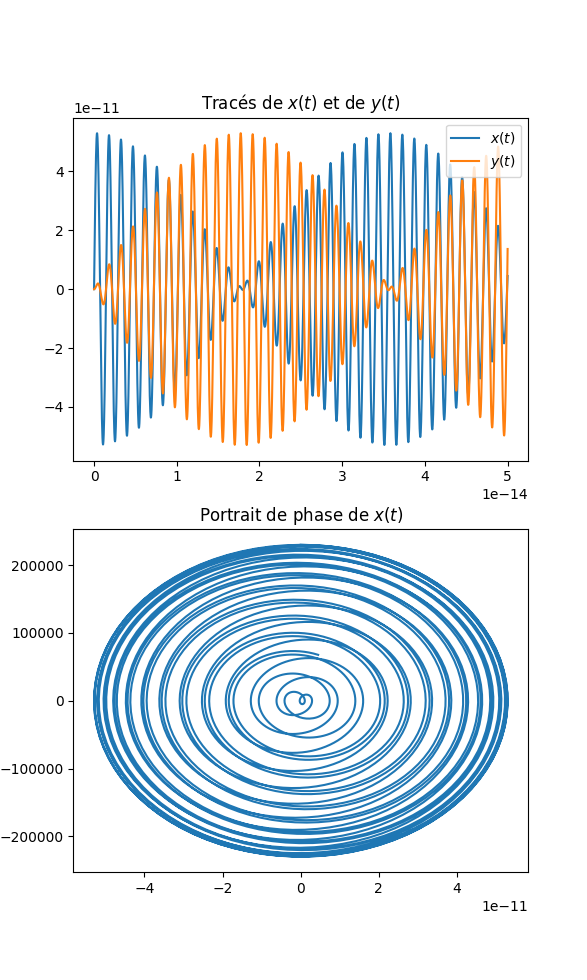
\includegraphics[width=8cm]{euler_vect_zeeman}    
\end{center}
\end{minipage}
%-------------------------------------------------------------------------------
\newpage
%--------------------------------------------------------------------------
\section{Sujets d'oraux de l'épreuve Centrale 2}
%--------------------------------------------------------------------------
%--------------------------------------------------------------------------
\begin{Exercise}\it
 On considère l’équation différentielle  $(1 - x)^3y''= y$.
 $f$ est la solution sur $]-\infty; 1[$.
 
En utilisant la méthode d’Euler, tracer une approximation du graphe de $f$ sur [0; 0,9].
\end{Exercise}
%--------------------------------------------------------------------------
\begin{Answer}

\end{Answer}
%--------------------------------------------------------------------------
%--------------------------------------------------------------------------
\begin{Exercise}\it 
On pose, pour tout $t\ne 0,$ 
$$A(t)=\begin{pmatrix}1-\frac1t & 1 \\ \frac{1}{2t} & 0 \end{pmatrix} \text{ et } (S)\left\{\begin{array}{l} x'(t)=\left(1-\frac1t \right)x(t)+y(t)\\ y'(t)=\frac{x(t)}{2t}\end{array}\right.$$
%--------------------------------------------------------------------------
\begin{enumerate}
\item Résoudre numériquement pour plusieurs valeurs de $x(1) = a$ et $y(1)=b$ , les tracer pour $t\in[1,4]. $ Commenter.
%--------------------------------------------------------------------------
\item {\bf Pour les cubes} : Pour $t\in\{0,5 ; 1 ; 1,5 ; 2\}, $ trouver les valeurs propres et des vecteurs propres de $A(t)$. Que peut-on conjecturer ?
\end{enumerate}
\end{Exercise}
%--------------------------------------------------------------------------
\begin{Answer}

\end{Answer}
%--------------------------------------------------------------------------
%--------------------------------------------------------------------------
\begin{Exercise}\it 
\begin{enumerate}
\item On considère l'équation $(E) : (1 - x)y'' = y$ sur $]-\infty,1[$.
\begin{enumerate}
\item Montrer qu'il existe une unique solution de $(E)$ sur $]-\infty,1[$ vérifiant $f(0) = 0$ et $f'(0) = 1$.
\item Représenter graphiquement $f$ sur $[-2;0,95]$.
\end{enumerate}

\item Soit $(a_n ) \in \R^{\N}$, définie par : $a_0 = 0,a_1 = 1$ 

et, pour tout $n\in \N -\{0,1\}$, $\displaystyle a_n = \frac{n-2}{n}a_{n-1} +  \frac{1}{n(n-1)}a_{n-2}$.
\begin{enumerate}
\item Représenter graphiquement $a_n $ pour $n\in [\![0,100]\!]$.
\item Montrer que le rayon de convergence de $\sum a_n x^n$ est supérieur ou égal à 1.
\item Représenter graphiquement $s : x\mapsto \sum\limits_{k=0}^{100}a_kx^k$ sur $[-1,1;0,95]$. Que constate-t-on ? 
\item Démontrer le résultat.
\end{enumerate}
\end{enumerate}
\end{Exercise}
%--------------------------------------------------------------------------
% \begin{Answer}
% \begin{enumerate}
% \item On pose $Y(x)=\left(\begin{array}{c} y(x)\\y'(x)\end{array}\right),$ ainsi $Y'(x)=\left(\begin{array}{c} y'(x)\\y''(x)\end{array}\right)=\left(\begin{array}{cc} 0&1\\\frac{1}{1-x}&0\end{array}\right)
% \left(\begin{array}{c} y(x)\\y'(x)\end{array}\right)$.

% On pose $f(Y,x)=\left(\begin{array}{c} Y[1]\\Y[0]/(1-x)\end{array}\right)$.
% On utilise ensuite {\tt import scipy.integrate as integr} puis {\tt integr.odeint}.
% \item 
% \end{enumerate}

% \begin{lstlisting}
% '''(1-x**2)y''=y, y(0)=0, y'(0)=1'''
% def feqDiff(Y,x) :
%   return(np.array([Y[1],Y[0]/(1-x)]))
% def traceSoluss(y0,yPrime0,b) :
%   '''trace une solution approchee sur [0,b]'''
%   N=1000
%   X=[ k*b/N for k in range(N)]
%   Y=integr.odeint(feqDiff, np.array([y0,yPrime0]), X)
%   plt.plot(X,Y[:,0]) # Y possede N lignes, 2 colonnes
%   plt.show()
%   return(Y)

% def traceEuler(y0,yPrime0,b) :
%   '''trace une solution approchee sur [0,b] avec Euler'''
%   N=1000
%   X=[ k*b/N for k in range(N)]
%   h=b/N
%   Y=[[y0,yPrime0]]
%   for k in range(1,N) :
%     Y.append([Y[k-1][0]+h*Y[k-1][1],Y[k-1][1]+h*Y[k-1][0]/(1-X[k-1])])
%   Y=np.array(Y)
%   #Ybis=integr.odeint(feqDiff, np.array([y0,yPrime0]), X)
%   plt.plot(X,Y[:,0]) # Y possede N lignes, 2 colonnes
%   #plt.plot(X,Ybis[:,0])
%   plt.show()
%   return(Y)
% \end{lstlisting}


% L'énoncé demande de tracer sur $[-2,0.95],$ on fait donc une méthode d'Euler avec un pas négatif, il ne faut pas oublier de retourner la liste avant de l'utiliser pour le graphe. On trace sur $[0,0.95]$ puis on reprend pour $[-2,0]$.


% \begin{lstlisting}
% def traceEulerbis(y0,yPrime0,a,b) :
%   '''trace une solution approchee sur [a,b] avec Euler'''
%   N=1000
%   X=[ k*b/N for k in range(N)]
%   h=b/N
%   Y=[[y0,yPrime0]]
%   for k in range(1,N) :
%     Y.append([Y[k-1][0]+h*Y[k-1][1],Y[k-1][1]+h*Y[k-1][0]/(1-X[k-1])])
%   Y=np.array(Y)
%   plt.plot(X,Y[:,0])
%   #on trace ensuite sur [a,0] avec un pas <0
%   X=[a- k*a/N for k in range(N)]
%   h=a/N
%   Y=[[y0,yPrime0]]
%   for k in range(1,N) :
%     Y.append([Y[k-1][0]+h*Y[k-1][1],Y[k-1][1]+h*Y[k-1][0]/(1-X[k-1])])
%   Y.reverse()
%   Y=np.array(Y)
%   plt.plot(X,Y[:,0])           
% \end{lstlisting}
% \end{Answer}
%-------------------------------------------------------------------------------
%--------------------------------------------------------------------------
\subsection{Un sujet de physique}
%--------------------------------------------------------------------------
%--------------------------------------------------------------------------
Ce sujet discute d’un modèle d’interaction forte, une force attractive s’exerçant seulement à courte distance entre
nucléons (protons et neutrons). On étudie en particulier l’interaction d’un neutron projectile de masse $m_n$ dont la trajectoire rencontre celle d’un noyau fixe, sphérique de rayon $r_0$. La trajectoire initiale du neutron est rectiligne uniforme de vitesse $v_0$ et de paramètre d’impact $y_0$.

Les données numériques dutilisent pour unités de longueur, d’énergie et de masse respectivement le femtomètre ($1 fm = 1,0 \times 10^{-15}m$), le méga-électron volt ($e = 1,60 \times 10^{-19} C$) et la masse d’un nucléon ($m_n = 1,67 \times 10^{-27} kg$)
%--------------------------------------------------------------------------
%--------------------------------------------------------------------------
\begin{Exercise}\it
Quelles sont les unités de durée et de vitesse correspondante ?
\end{Exercise}
%--------------------------------------------------------------------------
\begin{Answer}

\end{Answer}
%--------------------------------------------------------------------------
%--------------------------------------------------------------------------

\medskip

La force exercée par le noyau sur le neutron est centrale, attractive, d’expression (en coordonnées sphériques)
$\displaystyle \vec F = F(r)\vec e_r$ avec $\displaystyle  F(r) = -\frac{U_0}d \exp\left(-\frac{(r - r_0)^2}{d^2}\right)$ .
On donne
\begin{lstlisting}
U0 = 10.0
r0 = 1.0
d = .1
\end{lstlisting}
%--------------------------------------------------------------------------
%--------------------------------------------------------------------------
\begin{Exercise}\it
Tracer et interpréter les courbes donnant $F(r)$ et l’énergie potentielle $U(r)$ associée.
\end{Exercise}
%--------------------------------------------------------------------------
\begin{Answer}
\end{Answer}
%--------------------------------------------------------------------------
%--------------------------------------------------------------------------
% %--------------------------------------------------------------------------
% %--------------------------------------------------------------------------
% %--------------------------------------------------------------------------
% %--------------------------------------------------------------------------
% %--------------------------------------------------------------------------
% %--------------------------------------------------------------------------
% %--------------------------------------------------------------------------
% %--------------------------------------------------------------------------
% %--------------------------------------------------------------------------
% %--------------------------------------------------------------------------
% %--------------------------------------------------------------------------
% %--------------------------------------------------------------------------
% %--------------------------------------------------------------------------
% %--------------------------------------------------------------------------
% %--------------------------------------------------------------------------
% %--------------------------------------------------------------------------
% %--------------------------------------------------------------------------
% %--------------------------------------------------------------------------
% %--------------------------------------------------------------------------
% %--------------------------------------------------------------------------
% %--------------------------------------------------------------------------
% %--------------------------------------------------------------------------
% %--------------------------------------------------------------------------
% %--------------------------------------------------------------------------
% %--------------------------------------------------------------------------
% %--------------------------------------------------------------------------
% %--------------------------------------------------------------------------
% %--------------------------------------------------------------------------
% %--------------------------------------------------------------------------
% %--------------------------------------------------------------------------
% %--------------------------------------------------------------------------
% %--------------------------------------------------------------------------
% %--------------------------------------------------------------------------
% %--------------------------------------------------------------------------
% %--------------------------------------------------------------------------
% %--------------------------------------------------------------------------
% %--------------------------------------------------------------------------
% %--------------------------------------------------------------------------
% %--------------------------------------------------------------------------
% \newpage
% % %-------------------------------------------------------------------------------
% \section{Systèmes d'équations d'ordre 2}
% %-------------------------------------------------------------------------------
% %-------------------------------------------------------------------------------
% Lorsqu'un système différentiel est composé d'équation d'ordre 2, on le transforme en un système d'équations d'ordre 1 en doublant le nombre de variables : chaque variable est associée à sa dérivée.
% \subsection{Ceintures de Van Halen}
% %-------------------------------------------------------------------------------
% %-------------------------------------------------------------------------------
% Les ceintures de Van Halen sont des région autour de la terre dans lesquelles les particules chargées issues du soleil peuvent se retrouver piégées. Le champ magnétique terrestre dévie les particules de leur trajectoire vers la terre en leur faisant suivre les lignes de champ. Nous allons observer les trajectoire des protons dans la première ceinture située approximativement à une distance de 2 rayons terrestres du centre de la terre. On donne les valeurs 
% \begin{lstlisting}
% q0 = 1.6e-19 # C
% m0 = 1.67e-27 # kg
% \end{lstlisting}



% Le champ magnétique terrestre peut être approché par un dipole magnétique  : il est représenté son origine $O$, au centre de la terre par son moment magnétique $\vec \mu$ dont la direction est broche de l'axe de la terre. La valeur numérique estimée est $\|\vec \mu\| = 7,7.10^{22}\text{A}\cdot \text{s}^{-2}$.

% Les vecteurs dans {\sc Python} seront représentés par un tableau {\sc numpy} avec la troisième coordonnée indiquant l'axe de la terre
% \begin{lstlisting}
% mu = np.array([0.0, 0.0, 7.7e22])
% \end{lstlisting}



% Le champ magnétique en un point $M$ est alors, en notant $r = \left\|\overrightarrow{OM}\right\|$ et $\displaystyle \vec u = \frac 1 r\overrightarrow{OM}$,
% \[\overrightarrow{B(M)} = \frac{\mu_0}{4\pi}\frac{3(\vec \mu.\vec u)\vec u - \vec \mu}{r^3}\]
% On a $\mu_0=4\pi10^{-7}\text{kg}\cdot\text{m}\cdot\text{A}^{-2}\cdot\text{s}^{-2}$ et on notera \type{mu0} la valeur de $\displaystyle \frac{\mu_0}{4\pi}$ : \type{mu0 = 1.0 e-7}.

% Le produit scalaire de deux vecteurs représentés par des tableaux \type{u} et \type{v} de même taille se calcule par \type{np.dot(u, v)}, leur produit vectoriel par \type{np.cross(u, v)}

% %-------------------------------------------------------------------------------
% %-------------------------------------------------------------------------------
% \begin{Exercise}\it
% Écrire une fonction \type{B(M)} qui calcule le champ magnétique en un point $m$ représenté par un tableau {\sc numpy} de taille 3 (il représente aussi le vecteur $\overrightarrow{OM}$). 
% \end{Exercise}
% %--------------------------------------------------------------------------
% \begin{Answer}
% \begin{lstlisting}
% def B(M):
%     r = Norme(M)
%     u = (1/r)*M
%     return mu0*(3*np.dot(mu,u)*u -mu)/(r**3)
% \end{lstlisting}
% \end{Answer}
% %--------------------------------------------------------------------------
% %--------------------------------------------------------------------------
% L'équation différentielle dont on cherche les solution est alors
% \[m\frac{\overrightarrow{\d^2 M}}{\d t^2} = q\frac{\overrightarrow{\d M}}{\d t}\wedge \overrightarrow{B(M)}\]
% Cette équation va se traduire en un système différentiel à 6 variables : les 3 coordonnées de $x$, $y$ et $z$, coordonnées de $M$, et les coordonnées du vecteur vitesse. 
% %-------------------------------------------------------------------------------
% %-------------------------------------------------------------------------------
% \begin{Exercise}\it
% Écrire une fonction \type{psi(u, t)} qui décrit le système différentiel, elle reçoit deux variables, un tableau de taille 6 et un flottant pour le temps (qui n'intervient pas) et doit renvoyer un tableau de taille 6.  
% \end{Exercise}
% %--------------------------------------------------------------------------
% \begin{Answer}
% \begin{lstlisting}
% def phi(u, t):
%     M = u[0:3]
%     V = u[3:6]
%     dM = np.zeros(6)
%     dM[0:3] = V
%     dM[3:6] = q0*np.cross(V, B(M))/m0
%     return dM
% \end{lstlisting}
% \end{Answer}
% %-------------------------------------------------------------------------------
% %-------------------------------------------------------------------------------
% Les unités de base sont le rayon de la terre pour la position initiale et une fraction de la vitesse de la lumière pour la vitesse initiale. Par exemple :
% \begin{lstlisting}
% RT = 6.4e6
% c = 3.0e8
    
% u0 = np.array([0, 1*8*RT, 0, 0, 0.3*c, 0.15*c])
% \end{lstlisting}
% %-------------------------------------------------------------------------------
% %-------------------------------------------------------------------------------
% \begin{Exercise}\it
% Tracer la courbe intégrale d'une solution sur $[0; 3]$.

% Avec \type{odeint} le temps de calcul peut être long.
% \end{Exercise}
% %--------------------------------------------------------------------------
% \begin{Answer}
% \begin{lstlisting}
% T = np.linspace(0,3,20000)
% U= odeint(phi, u0, T)
% X = U[ : , 0]
% Y = U[ : , 1]
% Z = U[ : , 2]

% fig=plt.figure()
% ax=Axes3D(fig)
% ax.plot(X, Y, Z)
% plt.show()
% \end{lstlisting}
% \end{Answer}
% %--------------------------------------------------------------------------
% %--------------------------------------------------------------------------
% \begin{center}
% \includegraphics[width=14cm]{TP13_VanHalen}    
% \end{center}
% %--------------------------------------------------------------------------
% On peut souhaiter représenter la terre pour voir la position relative de la trajectoire.
% \begin{lstlisting}
% r = np.linspace(0, RT, 30)
% phi = np.linspace(0, 2*np.pi, 20)
% R, Phi = np.meshgrid(r, phi)
% X1 = R*np.cos(Phi)
% Y1 = R*np.sin(Phi)
% Z1 = (RT**2 - R**2)**0.5
% ax.plot_wireframe(X1, Y1, Z1, color = "gray")
% ax.plot_wireframe(X1, Y1, -Z1, color = "gray")
% ax.set_xlim([-d*1.1, d*1.1])
% ax.set_ylim([-d*1.1, d*1.1])
% ax.set_zlim([-1.2*RT, 1.2*RT])
% plt.show()
% \end{lstlisting}
% \type{meshgrid} construit deux tableaux à deux dimension à partir de deux tableaux à une dimension en répétant les valeurs sur les colonnes pour le premier tableau et sur les lignes pour le second.
% \begin{lstlisting}
% >>> np.meshgrid([1, 2, 3], [4, 5, 6])
% [array([[1, 2, 3],
%         [1, 2, 3],
%         [1, 2, 3]]),
%  array([[4, 4, 4],
%         [5, 5, 5],
%         [6, 6, 6]])]
% \end{lstlisting}
% %--------------------------------------------------------------------------
% \begin{center}
% \includegraphics[width=14cm]{TP13_VanHalen_terre}    
% \end{center}
% %--------------------------------------------------------------------------





